% !TEX root = 00_MAIN.tex

\chapter{GCP-SGD} \label{sec:gcp}

Kolda and Hong~\cite{KH19} propose using a stochastic gradient
descent method to solve the Generalized Canonical Polyadic (CP)
optimization of Equation~\ref{eq:gcp}.  This algorithm relies on samples
of the full sparse tensor to inexpensively estimate the loss function
$F$ and its gradient with respect to the model.

\section{Distributed-Memory Sampling} \label{sec:gcp_sample}

Uniform sampling of a large sparse tensor would likely select mostly zero
valued entries of the tensor, since the number of nonzeros in a sparse
tensor is much smaller than the number of zeros.
To ensure that a sufficient number of nonzeros of the sparse tensor are
selected in each sample, Kolda and Hong present
two sampling strategies:  stratified and semi-stratified.  
Stratified sampling samples $p$ nonzeros and $q$ zeros 
of $\X$ separately, allowing
sufficient numbers of nonzeros to be selected.  Semi-stratified sampling
samples $p$ nonzeros and $q$ tensor indices separately; 
tensor indices include both
nonzeros and zeros.  A correction to the partial derivative 
computation accounts
for the possibility that a sampled tensor index may actually be a nonzero.
All sampling is done ``with replacement''; that is, a nonzero or zero
may be selected and stored more than once.

Distributed-memory parallelism introduces some challenges to effective sampling.
Sampling nonzeros is straightforward; each processor $z$ samples some number 
$p_z$ of its locally stored nonzeros.
Sampling zeros is more challenging because, for sparse tensors, only 
nonzeros are explicitly stored.
In theory, each processor $z$ could simply sample $q_z$ 
indices from the index space of the entire tensor.  
In practice, however, this approach has severe parallel performance problems.
Stratified sampling of zeros, for example, 
requires a check for each selected index to
confirm that it is actually a zero, not a nonzero.
In parallel, this check would require all-to-all communication of all 
sampled indices to determine whether they are nonzeros on any processor.
Even in semi-stratified sampling, which doesn't require a check to 
confirm that sampled indices are truly zeros, sampling from the entire tensor
can cause performance problems, as the resulting set of indices can require
factor matrix entries from all processors for model and MTTKRP computation.
Restricting the domain from which each processor samples zeros can alleviate
both problems.

While the CP-ALS algorithm in GentenMPI can operate with an arbitrary 
distribution of the sparse tensor, for GCP-SGD, we restrict the distribution
so that each processor owns a unique ``bounding box'' of the tensor's
index space.  Processors' bounding boxes may not overlap, and they must cover
the entire index space of the tensor.  Thus, each processor is responsible
for both the nonzeros and zeros of a subtensor within the tensor.

Two bounding box options are available in GentenMPI.  The first arises from
the SPLATT medium-grain distribution~\cite{SK16} from 
Figure~\ref{fig:medgrain}.  In this distribution, every processor has an 
equal number of nonzeros, but an unequal number of zeros.  
To sample $p$ nonzeros uniformly across $P$ processors, $p_z$ is chosen
to be $p /P$ on every processor $z$.  For load balancing, then, one would want
every processor to use the same value of $q_z$ as well, giving 
an equal number of indices $p_z + q_z$ on each processor.
However, because bounding boxes are not uniformly sized
with a medium-grain distribution, achieving load balance causes the space
of zeros to be sampled nonuniformly, with the density of sampled zeros
being higher in small bounding boxes than in large ones.  Conversely,
scaling $q_z$ to the size of the bounding box results in imbalanced
numbers of sampled indices across processors.

An alternative is to use uniformly sized bounding boxes for each processor,
as in Figure~\ref{fig:uniformbox}.  This nearly trivial distribution of the
tensor's index space results in processors having unequal numbers of nonzeros
and zeros, but equal number of indices overall.  Thus, to achieve load balance,
each processor $z$ selects $s_z = (p+q)/P$ samples.  On processor $z$ with
$n_z$ nonzeros out of $n$ nonzeros in the tensor, the number of 
nonzeros samples $p_z$ is $p(n_z / n)$; the number of zero samples
$q_z$ is $s_z - p_z$.  
In this way, the numbers of indices per processor in the sampled tensor 
are balanced, and sampling of both zeros and nonzeros is done uniformly 
across the entire tensor.
As a practical consideration,
limits are imposed to ensure that $p_z$ is at least $0.1 (s_z)$ and 
no more than $0.9 (s_z)$; these limits ensure that both nonzeros and 
zeros are sampled even when the distribution of nonzeros to boxes is very 
imbalanced (e.g., when $p(n_z / n) > s_z$).

\begin{figure}[ht]
   \centering
   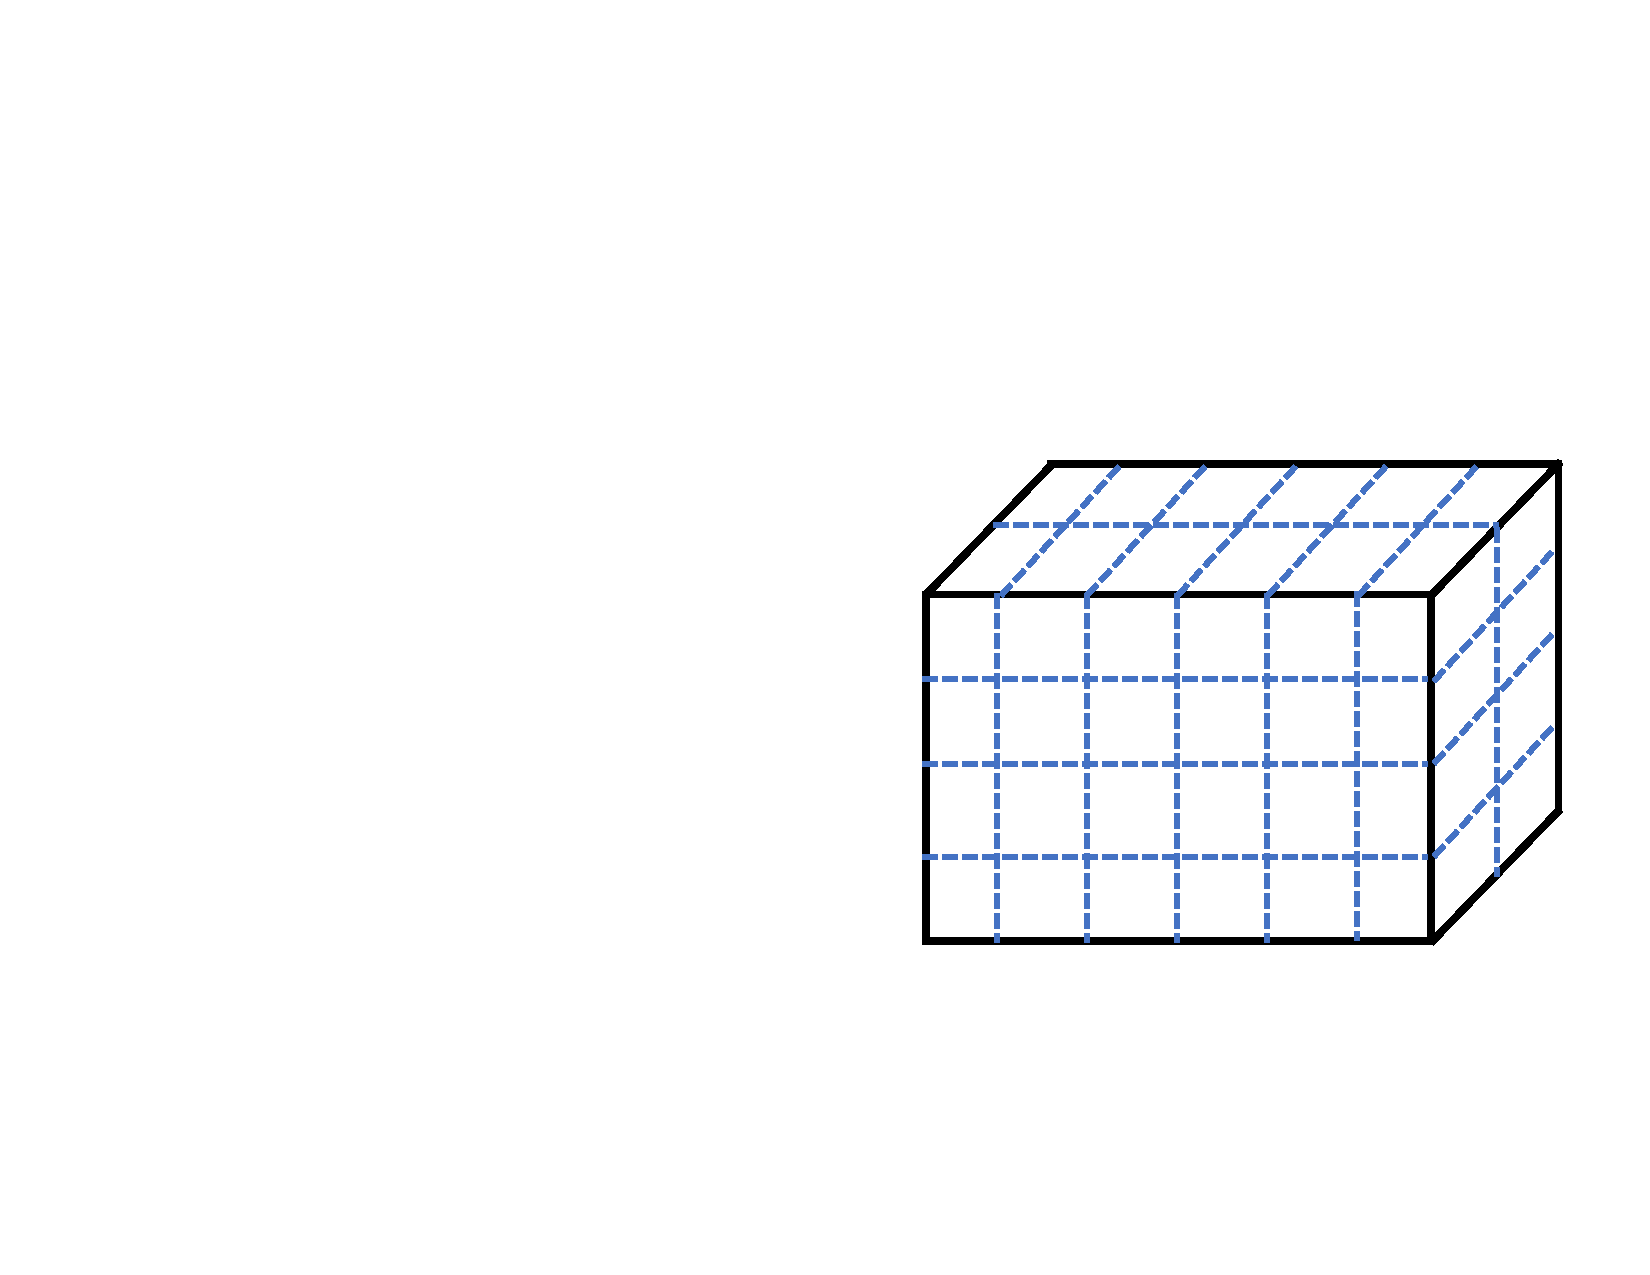
\includegraphics[keepaspectratio=true, width=2.5in]{figs/uniformbox}
   \caption[Uniformly sized box tensor distribution]{Illustration of a uniformly sized box distribution 
 of a three-way tensor to 48 processors}
   \label{fig:uniformbox}
\end{figure}

When using a sampled tensor to estimate the loss function, 
Kolda and Hong~\cite{KH19} scale the contributions of selected
zeros and nonzeros by a factor that amplifies the contribution based on sample
size.  For stratified sampling, they define the estimated loss function 
$\hat F$ (Equation 5.2 of~\cite{KH19}) as 

$$\hat F \equiv \sum_{x_{ijk} \ne 0} \frac{n}{p} f(x_{ijk},m_{ijk}) + 
                \sum_{x_{ijk} = 0} \frac{(N-n)}{q} f(0, m_{ijk}) $$

where the summations are over sampled tensor entries only,
$N$ is the total number indices in the tensor (i.e., the product
of the tensor dimensions), $n$ is the number of tensor nonzeros, $p$ is
the number of nonzeros samples, and $q$ is the number of zero samples.
In distributed memory with local sampling, we locally scale the contributions 
of each index before summing over all processors:
\begin{equation}
\hat F \equiv \sum_{\text{all processors } z} \text{       }
   \sum_{x_{ijk} \ne 0} \frac{n_z}{p_z}  f(x_{ijk},m_{ijk}) +
   \sum_{x_{ijk} = 0} \frac{(N_z-n_z)}{q_z} f(0, m_{ijk})
\label{eq:localloss}
\end{equation}

where the inner summations are over sampled entries, and, on processor $z$, 
$N_z$ is the number of indices in the bounding box 
(i.e., the product of the bounding box dimensions), $n_z$ is the number of 
nonzeros, and $p_z$ and $q_z$ are the numbers of nonzero
and zero samples, respectively.



\section{Algorithm and Parallel Implementation} \label{sec:gcp_alg}

To solve the optimization 
problem in Equation~\ref{eq:gcp}, Kolda and Hong~\cite{KH19} adopt
the Adam optimization algorithm~\cite{KB15} outlined in 
Algorithm~\ref{alg:gcpadam}.
Here, we follow~\cite{KH19} and write the model $\M = [\lambda;\{A_k\}]$,
where $\{ A_k \}$ is the set of factor matrices making up the model.
(In our prior three-way examples, $\{A_k\} = \{A,B,C\}$.)
Algorithm parameters $\alpha$, $\beta_1$, $\beta_2$, $\epsilon$, $\tau$, and
$\nu$ are user-specified parameters controlling the learning rate of 
Adam; we use the default values from TensorToolbox~\cite{TensorToolbox}:
$\alpha=0.001$, $\beta_1=0.9$, $\beta_2=0.999$, $\epsilon=1e-8$, $\tau=1000$, 
and $\nu=0.1$.  Parameter $\ell$ is a lower bound of reasonable solution values
(e.g., $0$ for non-negative tensors).  

\begin{algorithm}
  %\setstretch{1.25}
  \caption{GCP-Adam}
  \label{alg:gcpadam}
  \begin{algorithmic}[1]
    \Function{GCP-Adam}{$\X$, $\M=[\lambda;\{ A_k \}]$, $s$, $\alpha$, $\beta_1$, $\beta_2$, $\epsilon$, $\tau$, $\nu$,  $\ell$}
    \State \label{alg:gcpsetup1} Randomly initialize $\{ A_k \}$
    \State \label{alg:gcpsetup2} $\{ T_k \} \gets 0$; $\{ U_k \} \gets 0$
    \Comment{temporary factor matrices for $\{ A_k \}$}
    \State \label{alg:gcpfsample} $\hat \X \gets $ sparse tensor stratified-sampled from $\X$
    \State \label{alg:gcpfest}$\hat F \gets \textsc{EstObj}(\hat \X, \{ A_k \})$
    \Comment{estimate loss with fixed set of samples}
    \State $t \gets 0$
    \Comment{$t=$ \# of Adam iterations}
    \While{max number of bad epochs not exceded}
    \State Save copies of $\{ A_k \}$, $\{ T_k \}$ and $\{ U_k \}$
    \Comment{save in case of failed epoch}
    \State $\hat F_{\text{old}} \gets \hat F$
    \Comment{save to check for failed epoch}
    \For{$\tau$ iterations}
      \Comment{$\tau = $ \# iterations per epoch}
      \State $\{ G_k \} \gets \textsc{StocGrad}(\X, \{ A_k \}, s)$
      \Comment{$s = $ \# samples per stochastic gradient}
      \For{$k = 1, |\{ A_k \}|$}\tikzmark{AdamTop}
        \State $t \gets t+1$
        \State \label{alg:gcpstart} $T_k \gets \beta_1 T_k + (1-\beta_1) G_k$ 
        \State $U_k \gets \beta_2 U_k + (1-\beta_2) G_k^2$
        \State $\hat T_k \gets T_k / (1-\beta_1^{t})$
        \State $\hat U_k \gets U_k / (1-\beta_2^{t})$
        \State $A_k \gets A_k - \alpha \cdot ( \hat T_k \oslash (\sqrt{\hat U_k}+\epsilon) )$\hspace{3mm}\tikzmark{AdamRight}\tikzmark{AdamBottom}
        \State \label{alg:gcpstop} $A_k \gets \max\{A_k, \ell\}$  
        \Comment{$\ell =$  lower bound}
      \EndFor
    \EndFor
    \State \label{alg:gcbupdatefest} $\hat F \gets \textsc{EstObj}(\hat \X, \{ A_k \})$  \Comment{estimate loss with fixed set of samples}
    \If{$\hat F > \hat F_{\text{old}}$} \Comment{check for failure to decrease loss}
    \State Restore saved copied of $\{ A_k \}$, $\{ T_k \}$, $\{ U_k \}$  \Comment{revert to last epoch's variables}
    \State $\hat F \gets \hat F_{\text{old}}$ \Comment{revert to prior function value}
    \State $t \gets t - \tau$ \Comment{wind back the iteration counter}
    \State $\alpha \gets \alpha \cdot \nu$ \Comment{reduce the step length}
    \EndIf
    \EndWhile
    \State \Return $\Akset$
    \EndFunction
  \end{algorithmic}
  \AddNote{AdamTop}{AdamBottom}{AdamRight}{7cm}{Adam update depends on $\beta_1$, $\beta_2$, $\epsilon$; $\alpha =$ learning rate}
\end{algorithm}


Temporary factor matrices $\{ T_k \}$ and $\{ U_k \}$ are created using the 
same parallel distribution (i.e., the same Tpetra {\tt Maps}) 
as $\{ A_k \}$.  Thus, the randomization and initialization in 
lines~\ref{alg:gcpsetup1}-\ref{alg:gcpsetup2} can be done locally on each
processor's portion of the factor matrices with
no communication.
Likewise, the element-wise factor-matrix operations in 
lines~\ref{alg:gcpstart}-\ref{alg:gcpstop}
can be performed locally; no communication is
needed.

The sparse tensor $\hat \X$ is used to estimate error during GCP-SGD.
It is constructed via stratified sampling using a fixed set of sampled 
indices.
Its creation in line~\ref{alg:gcpfsample} requires communication
to create its maps and import objects relative to $\{ A_k \}$.
The loss function computation in 
line~\ref{alg:gcpfest} requires ``expand'' communication to send the entries of
$\{ A_k \}$ corresponding to indices of $\hat \X$ 
as described Chapter~\ref{sec:mttkrp}; since $\hat \X$ contains zero indices
that were not in $\X$, processors need different factor matrix entries
than they needed for $\X$.  Similarly, expand communication is needed for 
line~\ref{alg:gcbupdatefest} as the entries of $\{ A_k \}$ were modified
by the loop above.

The stochastic gradient computation is by far the most expensive part of 
the GCP-Adam computation.  Algorithm~\ref{alg:sg} provides a high-level
overview of our parallel implementation; mathematical details for stratified
and semi-stratified computation are found in~\cite{KH19}, Algorithms 
4.2 and 4.3, respectively.

In line~\ref{alg:sgsptensor} of Algorithm~\ref{alg:sg}, 
a sampled tensor $\Y$ with $s$ samples is created via stratified or
semi-stratified sampling. The sampling itself is local to each processor, 
but creation of the sampled tensor requires communication to construct its 
maps in each mode.
In line~\ref{alg:sgsystem}, we 
build a {\tt distSystem} class to create the communication
pattern (import objects) between the $\Y$ and $\{ A_k \}$ and expand
values from $\{ A_k \}$ to processors that need them.
Again, $\Y$ may have a different set of zeros from $\X$ and $\hat \X$, so 
different maps and import objects are needed for $\Y$.
In line~\ref{alg:sgdfdm}, the sampled values in $\Y$ are overwritten by
the element-wise partial gradient tensor
such that
$y_{ijk} = \frac{\delta f}{\delta m}(x_{ijk}, m_{ijk})$.
Then MTTKRP operations (line~\ref{alg:sgmttkrp}) 
are used to compute the returned values $\{ G_k \}$.
Only ``fold'' communication of $\{  G_k \}$
is needed during MTTKRP as the values of $\{ A_k \}$
were communicated (expanded) 
during system construction and do not change in the MTTKRP.

Stochastic gradient implementations in TensorToolbox and Genten fuse 
sampling with the partial derivative computation.  They do not form a 
sampled tensor but, rather, sample an index and immediately compute
the element-wise derivative at the index, storing it in $\Y$. They can
do this fusion because they operate in a single memory space and have all 
factor matrix entries available for use.  Since GentenMPI operates in 
distributed memory, it does not have all factor matrix entries associated
with a given sampled index within a processor; those entries must be 
communicated.  We construct the sampled tensor, then, so that the 
communication can be done in one round rather than for each sampled index.



\begin{algorithm}
  \caption{StocGrad}
  \label{alg:sg}
  \begin{algorithmic}[1]
  \Function{StocGrad}{$\X$, $\{ A_k \}$, $s$}
  \State \label{alg:sgsptensor} Sample $s$ indices and construct sparse tensor $\Y$
  \State \label{alg:sgsystem} Build {\tt distSystem} object from $\Y$ and $\{ A_k \}$
  \State \label{alg:sgdfdm} $\Y \gets $ element-wise $\frac{\delta f}{\delta m}$
  \For{$A_m \in \{ A_k \}$}
    \State \label{alg:sgmttkrp} $G_m \gets $ MTTKRP($\Y$, $\{ A_k \} \backslash A_m$)
  \EndFor
  \State return $\{ G_k \}$
  \EndFunction
  \end{algorithmic}
\end{algorithm}


\section{Experimental Results} \label{sec:gcp_exp}

\subsection{Convergence Results}

In this section we present convergence results of GCP-SGD for three different data sets, each using a Poisson loss function and the semi-stratified sampling strategy.
\Cref{fig:chicago_conv,fig:lbnl_conv,fig:amazon_conv} plot the values of the loss function over time.
The first two datasets are small enough to run on a single node, and the first experiment is designed to be compared against an existing result using a MATLAB implementation of the GCP-SGD algorithm \cite{KH19}.
The third data set is too large for GCP-SGD to execute on a single node, and the experiment is performed using 16 nodes.

\begin{figure}
\renewcommand{\datafile}{data/convergence/chicago_conv.dat}
\centering
\begin{tikzpicture}
\begin{axis}[
	ylabel={Error (Poisson loss)}, 
	xlabel={Time (seconds)},
	ymax=2.3e7,
	ymin=2e7,
]
	\addplot table[x=Time, y=Error] {\datafile};    
\end{axis}
\end{tikzpicture}
\caption[GCP-SGD convergence for \emph{Chicago crime data} tensor]{GCP-SGD convergence results for Chicago crime data, using Poisson loss, rank $R=10$, and semi-stratified gradient sampling.  Each of the 92 markers corresponds to an epoch, each epoch corresponds to 1000 iterations, and each iteration used a total of 3152 nonzero samples and 3152 index (zero) samples.  The error is estimated using stratified objective function sampling with 31{,}588 nonzero samples and 31{,}596 zero samples.}
\label{fig:chicago_conv}
\end{figure}

\Cref{fig:chicago_conv} shows the convergence results for GCP-SGD on the \emph{Chicago crime} data set from the FROSTT \cite{FROSTT} collection using Poisson loss.
The Chicago crime data tensor is $6186\times 24\times 77\times 32$ with 5.3 million nonzeros.
This result can be compared against \cite[Figure 5.6]{KH19}, where the same GCP-SGD algorithm is used (with similar parameter settings) in a MATLAB environment.
In both cases, the Poisson loss converges to approximately \texttt{2.05e7}, though the time required is less for the parallel results.
The experiment was performed on a single node of Skybridge, with one MPI process for each of the 16 cores.
The average time per iteration is 1.24 seconds.

\begin{figure}
\renewcommand{\datafile}{data/convergence/lbnl_conv.dat}
\centering
\begin{tikzpicture}
\begin{axis}[
	ylabel={Error (Poisson loss)}, 
	xlabel={Time (seconds)},
]
	\addplot table[x=Time, y=Error] {\datafile};    
\end{axis}
\end{tikzpicture}
\caption[GCP-SGD convergence for \emph{LBNL network} tensor]{GCP-SGD convergence results for LBNL network data, using Poisson loss, rank $R=10$, and semi-stratified gradient sampling.  Each of the 30 markers corresponds to an epoch, each epoch corresponds to 1000 iterations, and each iteration used a total of 439{,}879 nonzero samples and 439{,}881 index (zero) samples.  The error is estimated using stratified objective function sampling with 4{,}398{,}859 nonzero samples and 4{,}398{,}869 zero samples.}
\label{fig:lbnl_conv}
\end{figure}

\Cref{fig:lbnl_conv} shows the convergence results for GCP-SGD on the \emph{LBNL network} data set from the FROSTT \cite{FROSTT} collection using Poisson loss.
The \emph{LBNL network} tensor is $1605 \times 4198 \times 1631 \times 4209 \times 868131 $ with 1.7 million nonzeros.
The experiment was performed on a single node of Skybridge, with one MPI process for each of the 16 cores.
The average time per iteration is 143 seconds.

Compared to the \emph{Chicago crime} data set, the \emph{LBNL network} data set takes over 100 times longer per iteration.
This is because the number of entries in the model is proportional to the sum of the tensor dimensions, and the number of samples used is chosen to be proportional to the number of entries in the model.
That is, the number of samples used for \emph{LBNL network} is about 100 times the number used for \emph{Chicago crime}, which helps to explain the increase in time.

\begin{figure}
\renewcommand{\datafile}{data/convergence/amazon_conv.dat}
\centering
\begin{tikzpicture}
\begin{axis}[
	ylabel={Error (Poisson loss)}, 
	xlabel={Time (seconds)},
]
	\addplot table[x=Time, y=Error] {\datafile};    
\end{axis}
\end{tikzpicture}
\caption[GCP-SGD convergence for \emph{amazon-reviews} tensor]{GCP-SGD convergence results for \emph{amazon-reviews} data, using Poisson loss, rank $R=16$, and semi-stratified gradient sampling.  Each of the 11 markers corresponds to an epoch, each epoch corresponds to 1000 iterations, and each iteration used a total of 4{,}200{,}196 nonzero samples and 4{,}200{,}444 index (zero) samples.  The error is estimated using stratified objective function sampling with 42{,}003{,}186 nonzero samples and 42{,}003{,}214 zero samples.}
\label{fig:amazon_conv}
\end{figure}


\Cref{fig:amazon_conv} shows the convergence results for GCP-SGD on the \emph{amazon-reviews} data set from the FROSTT \cite{FROSTT} collection using Poisson loss.
The experiment was performed on 16 nodes of Skybridge, with one MPI process per core, for a total of 256 MPI processes.
The average time per iteration is 869 seconds.

\subsection{Parallel Distribution for Sampling}

We compare the performance of Algorithm~\ref{alg:gcpadam} using the 
medium-grained distribution and uniform-box distributions described in
Section~\ref{sec:gcp_sample}.  For our experiments, we use the \emph{amazon-reviews}
tensor from the 
FROSTT~\cite{FROSTT} collection.
The Amazon data tensor is $4821207\times 1774269\times 1805187 $ with 1.7 billion nonzeros.
In Figure~\ref{fig:amazon_medgrain_vs_uniformbox}, we show execution times 
for five epochs with 1000 iterations each on
the Skybridge cluster with 128 to 2048 processors.  In all cases, the 
uniform-box distribution resulted in lower execution time and more consistent
scaling performance.  With the uniform-box distribution, less time
was needed for performing MTTKRP and building maps between the sampled tensor and factor matrices.

\begin{figure}
\centering
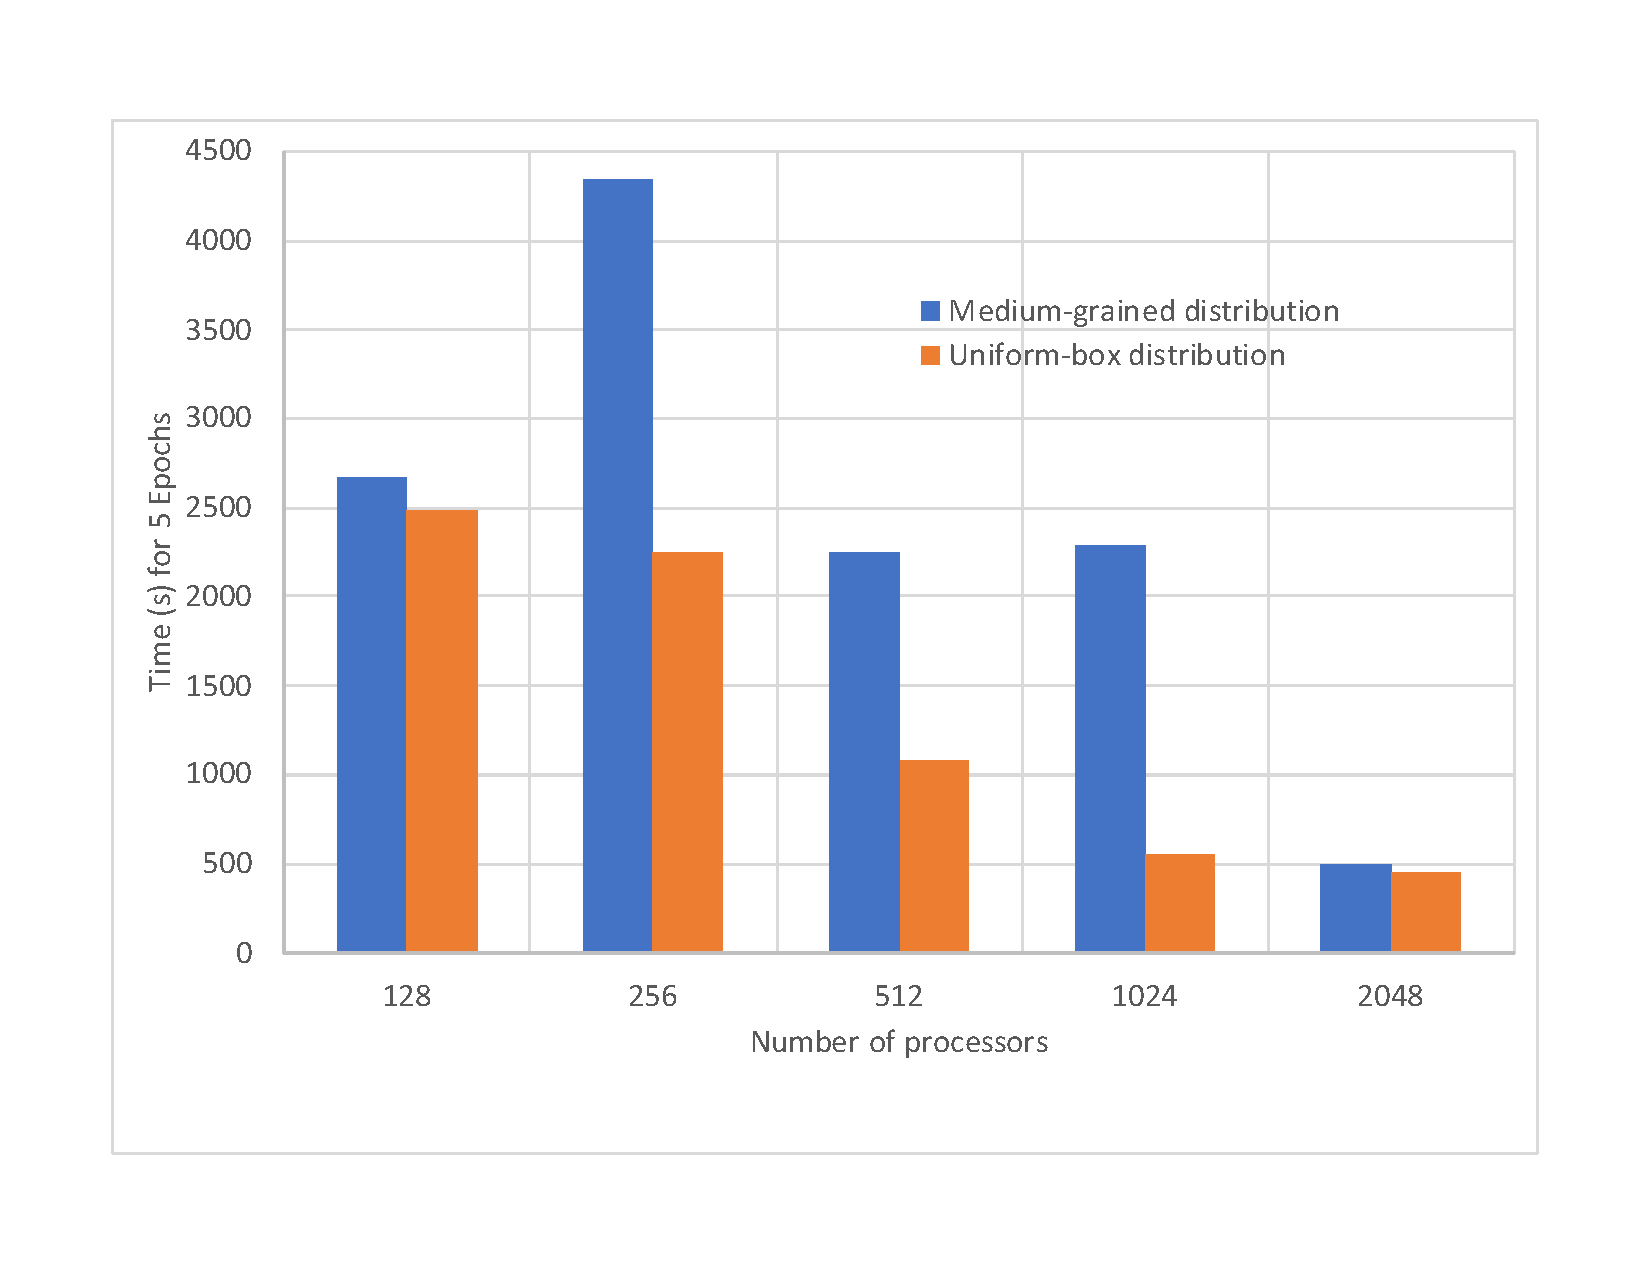
\includegraphics[keepaspectratio=true, width=4.5in]{figs/amazon_medgrain_vs_uniformbox}
\caption[Runtime comparison with medium-grained and uniform-box distributions]{Comparison of runtimes using the \emph{amazon-reviews} tensor using $L^2$ loss, rank $R=16$, and semi-stratified sampling using medium-grained partitioning versus a uniform box distribution.  
Each of the five epochs ran 1000 iterations.  
Each iteration used semi-stratified sampling with approximately 4.2M nonzeros and 4.2M zeros. 
Error estimation used stratified sampling with approximately 42M nonzeros and 42M zeros. 
}
\label{fig:amazon_medgrain_vs_uniformbox}
\end{figure}

Given the benefit of uniform-box distribution, we use it in all subsequent 
parallel experiments.

\subsection{Strong Scaling and Timing Breakdown}

Having confirmed the convergence behavior of GentenMPI, we now consider its parallel performance and strong scaling.
\Cref{fig:lbnl_scaling,fig:random_scaling,fig:amazon_scaling} demonstrate the strong scaling behavior for \emph{LBNL network}, random, and \emph{amazon-reviews} data sets.
All experiments were performed on Skybridge, and all used $L^2$ loss and the semi-stratified sampling strategy.

\begin{figure}
\centering
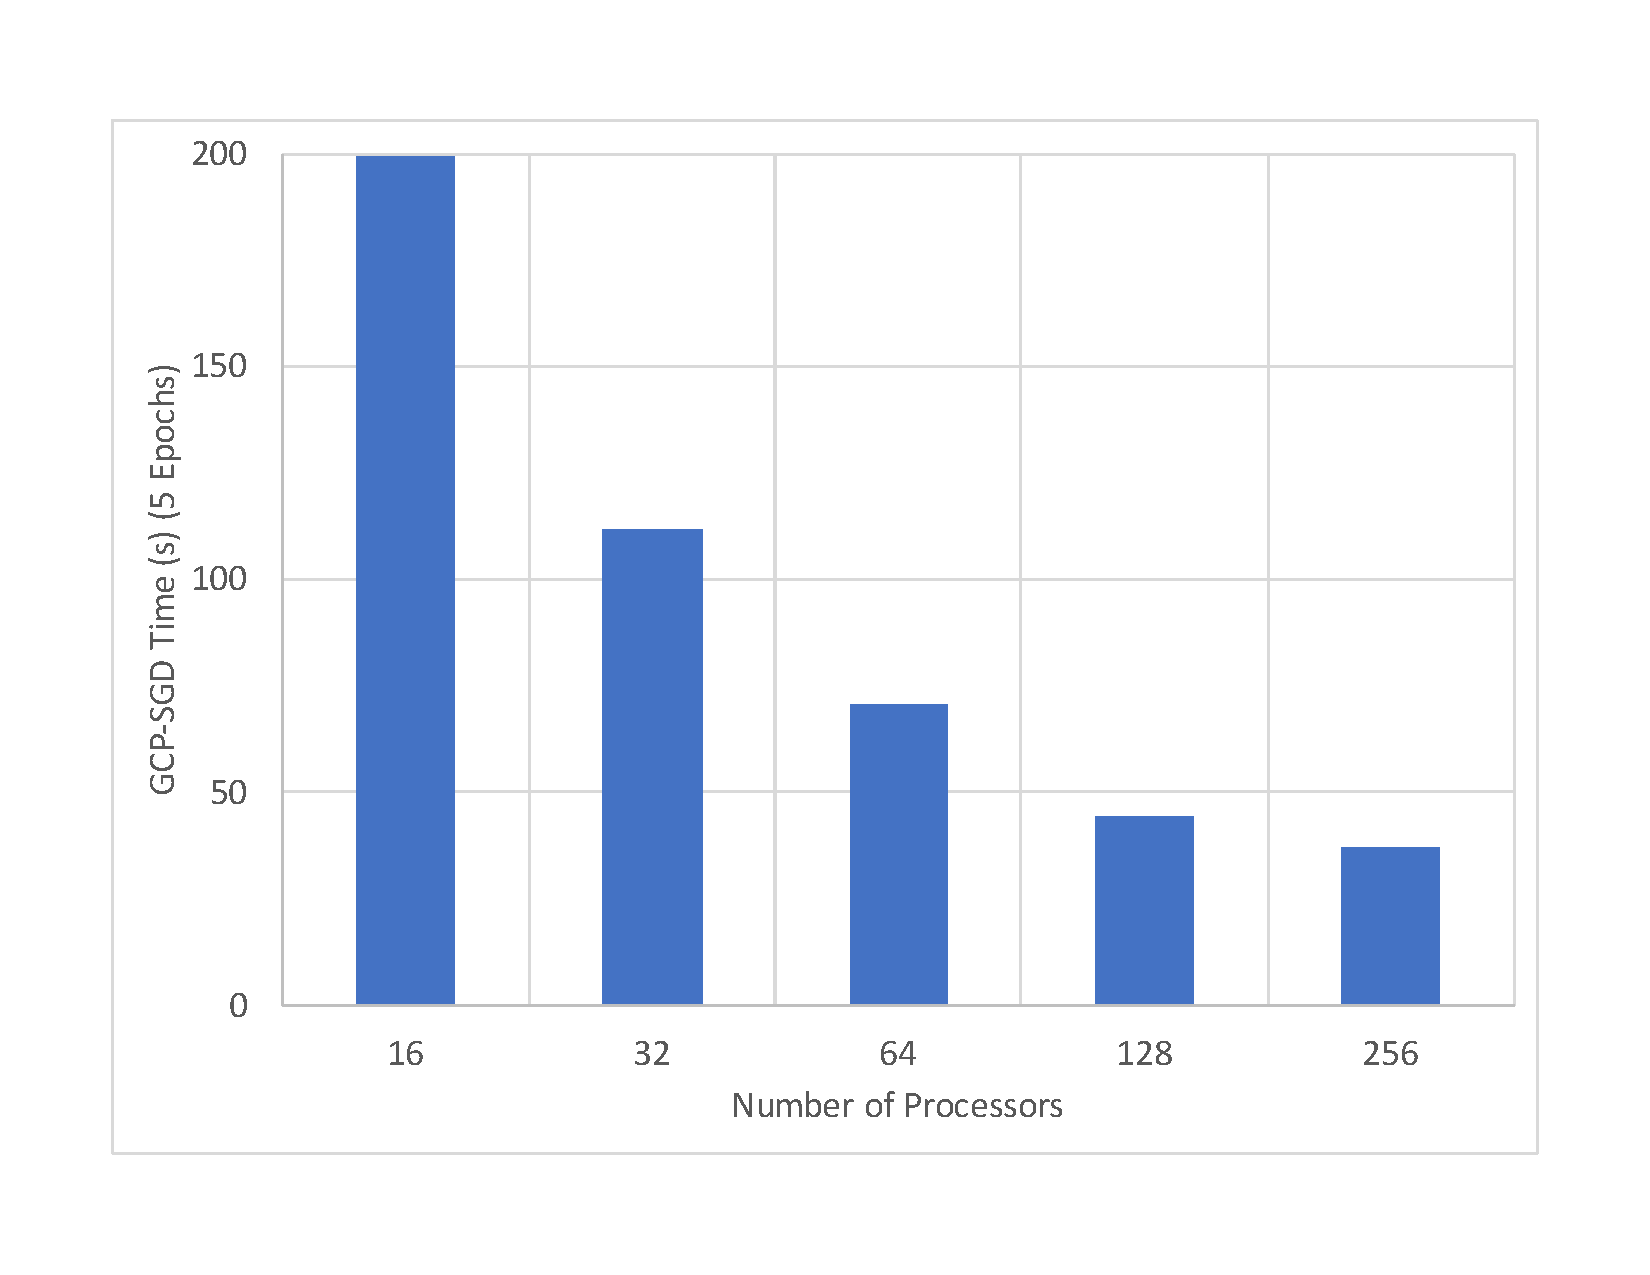
\includegraphics[keepaspectratio=true, width=4.5in]{figs/strongLBNL}
\caption[Strong scaling of GCP-SGD for \emph{LBNL network} tensor]{Strong scaling for \emph{LBNL network} tensor using $L^2$ loss, rank $R=16$, and semi-stratified sampling.  
Each of the five epochs ran 1000 iterations.  
Each iteration used semi-stratified sampling with approximately 10K nonzeros and 10K zeros. 
Error estimation used stratified sampling with approximately 100K nonzeros and 100K zeros. 
}
\label{fig:lbnl_scaling}
\end{figure}

The \emph{LBNL network} data set has order five, with about 1.7 million nonzeros.
For the experimental results in \Cref{fig:lbnl_scaling}, we use approximately 200{,}000 samples to estimate the error and 20{,}000 samples in the stochastic gradient tensor.
On 16 processors (1 node of Skybridge), the time for 5 epochs is 192 seconds.
For comparison, Genten \cite{PK19} takes between 101 and 120 seconds, depending on the MTTKRP implementation used.
The strong scaling is reasonable up to 128 processors, achieving over a $4\times$ speedup, but there is little reduction from 128 to 256 processors.
At 256 processors, the average number of original tensor nonzeros per processor is quite small --- less than 10{,}000 --- and the number of samples per processor is less than 100.

\begin{figure}
\centering
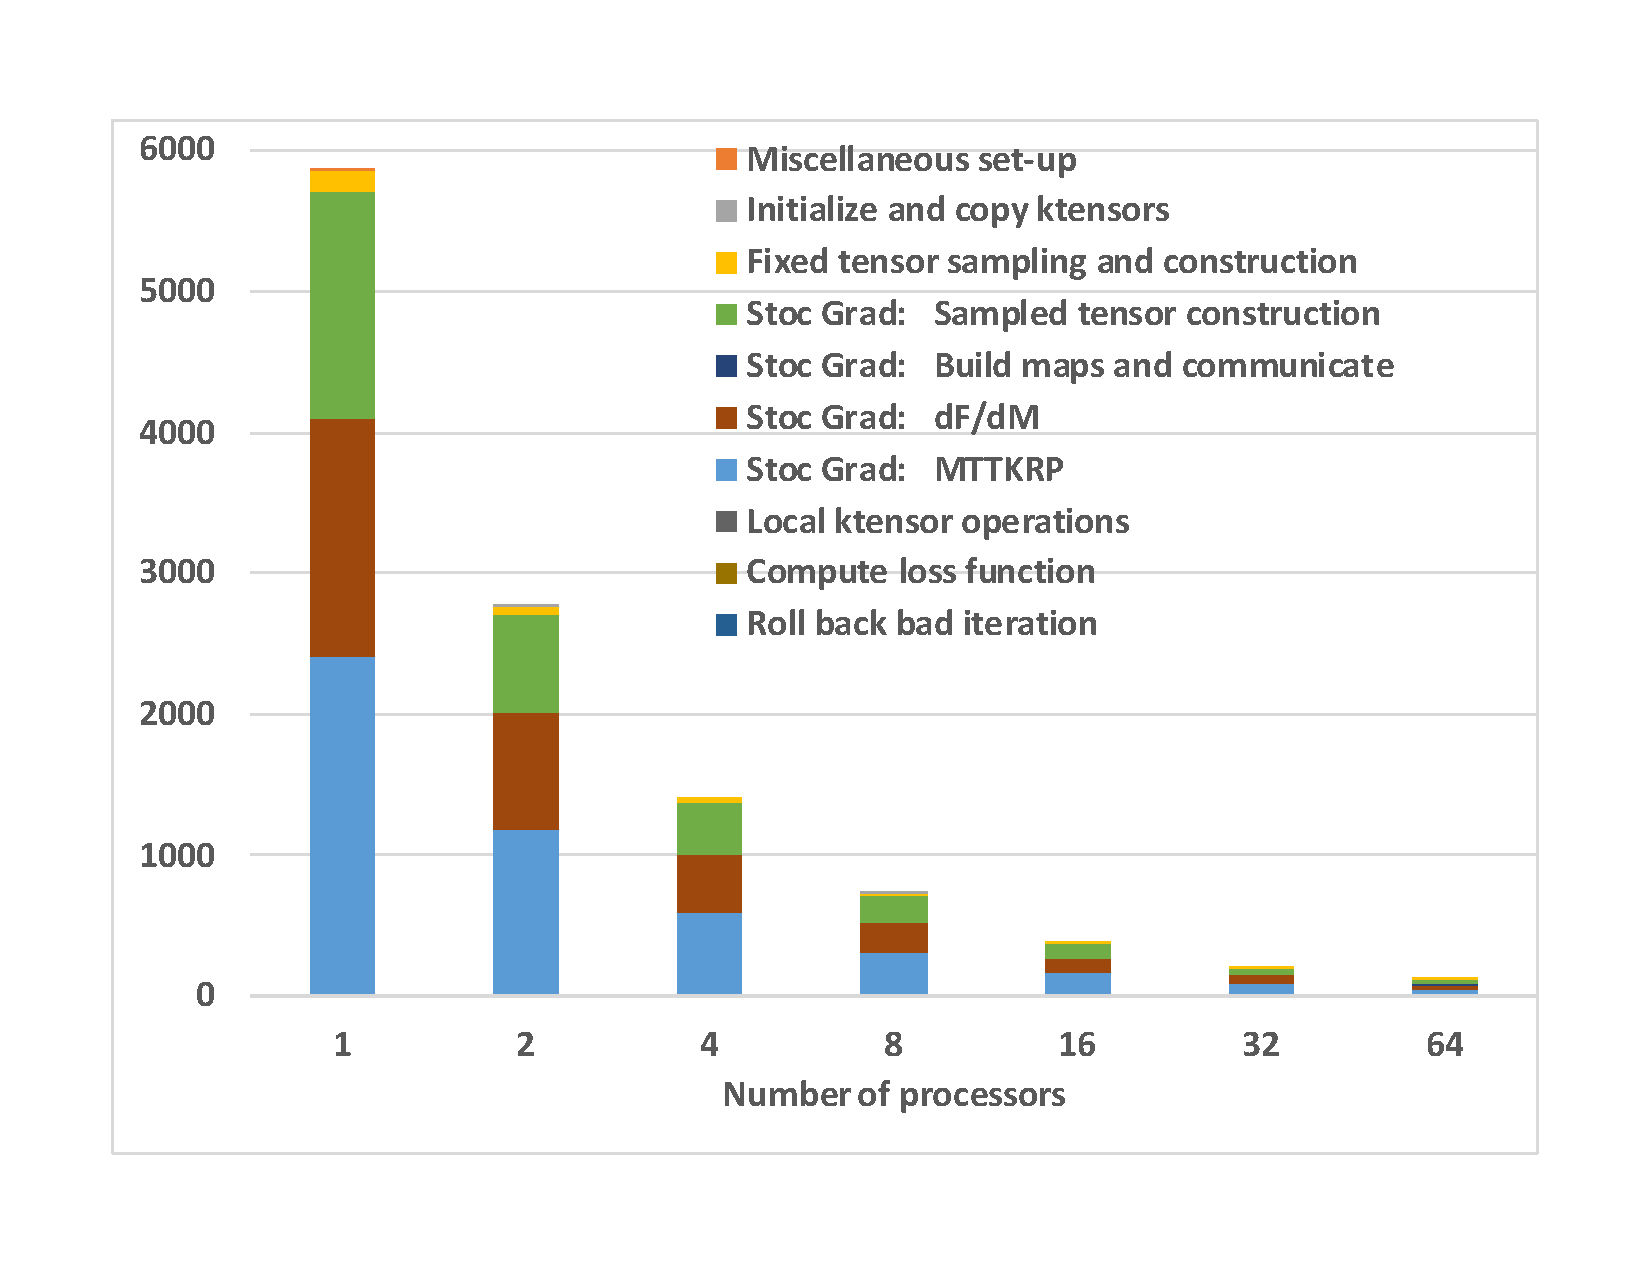
\includegraphics[keepaspectratio=true, width=4.5in]{figs/strongRandomStacked}
\caption[Strong scaling of GCP-SGD for random order-4 tensor]{Strong scaling for random 4D tensor using $L^2$ loss, rank $R=16$, and semi-stratified sampling.  
Each of the five epochs ran 1000 iterations.  
Each iteration used semi-stratified sampling with approximately 768K nonzeros and 768K zeros. 
Error estimation used stratified sampling with approximately 2.6M nonzeros and 2.6M zeros. 
}
\label{fig:random_scaling}
\end{figure}

\Cref{fig:random_scaling} shows experimental results for a random tensor, which allows for perfect load balance of nonzeros, even in the case of uniform boxes.
The random tensor is $1000\times 1000\times 500\times 500$ with 256 million nonzeros.
We use approximately 5 million samples to estimate the error and 1.5 million samples in each stochastic gradient.
Using 16 processors (1 node), GentenMPI took 373 seconds; Genten~\cite{PK19} with 16 threads took between 306 and 1250 seconds, depending on the MTTKRP implementation used.
From one MPI rank to 64 ranks, GentenMPI exhibited a $52.7\times$ speed-up.

From the time breakdown, we see that the dominant kernels in this experiment (using up to 64 processors) are within the stochastic gradient computation: evaluating the partial derivative, constructing the sampled tensor, and performing the MTTKRP.
No communication is needed to evaluate the partial derivative.  Similarly, no communication
is needed to sample the tensor, but a small amount of communication occurs in creating the
Tpetra maps describing the distribution of the sampled tensor 
(see Section~\ref{sec:sptensor}).  
The cost of building maps (the communication pattern) and performing the communication are small in this case, but they grow with the number of processors.

\begin{figure}
\centering
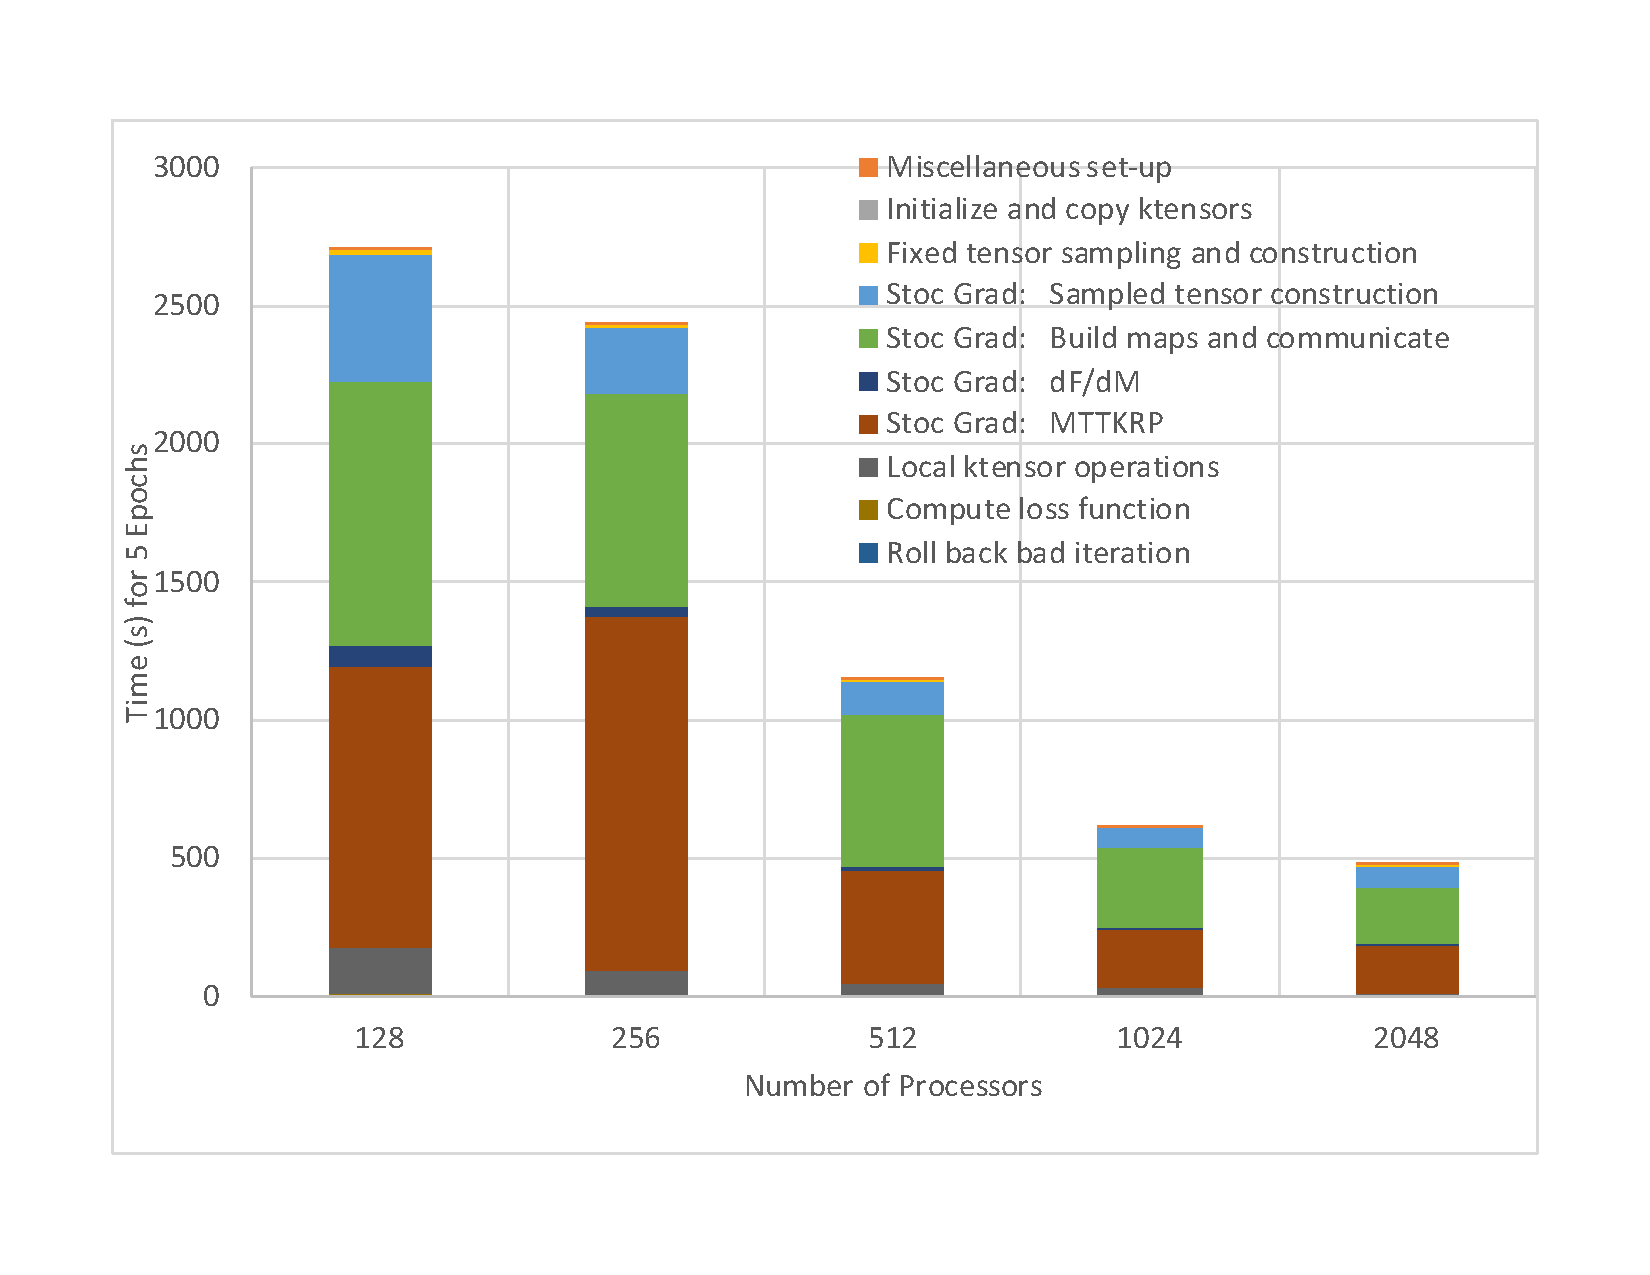
\includegraphics[keepaspectratio=true, width=4.5in]{figs/amazon_stacked}
\caption[Strong scaling of GCP-SGD for \emph{amazon-reviews} tensor]{Strong scaling for \emph{amazon-reviews} tensor using $L^2$ loss, rank $R=16$, and semi-stratified sampling.  
Each of the five epochs ran 1000 iterations.  
Each iteration used semi-stratified sampling with approximately 4.2M nonzeros and 4.2M zeros. 
Error estimation used stratified sampling with approximately 42M nonzeros and 42M zeros. 
}
\label{fig:amazon_scaling}
\end{figure}

\Cref{fig:amazon_scaling} presents results for the \emph{amazon-reviews} tensor, using between 128 and 2048 processors of Skybridge (the tensor is too large to run GCP-SGD on fewer processors).
We use 84 million samples to estimate the error and 8.4 million samples for each stochastic gradient.
Compared to the experiment with the random tensor, we see that communication costs become much more significant in this experiment.
The dominant kernels are again in the stochastic gradient computation, but in this case, the communication costs (building maps and communicating) are significant on 128 processors and become a bottleneck on 2048 processors.
The scaling is nearly perfect between 256 and 1024 processors, but little speedup is obtained in increasing to 2048 processors.
